\documentclass[aspectratio=169,14pt]{beamer}
\usepackage[T1]{fontenc}
\usepackage{lmodern}
\usepackage{booktabs}
\usepackage{listings}
\usepackage{pgfpages}
\usefonttheme{professionalfonts}

\definecolor{Navy}{HTML}{18334B}
\definecolor{Teal}{HTML}{087F8C}
\definecolor{Ink}{HTML}{253443}
\definecolor{Muted}{HTML}{526370}
\definecolor{Paper}{HTML}{F3F6F8}
\setbeamercolor{normal text}{fg=Ink,bg=white}
\setbeamercolor{structure}{fg=Teal}
\setbeamercolor{frametitle}{fg=Navy}
\setbeamercolor{title}{fg=Navy}
\setbeamercolor{footline}{fg=Muted}
\setbeamerfont{frametitle}{size=\Large,series=\bfseries}
\setbeamersize{text margin left=8mm,text margin right=8mm}
\setbeamertemplate{navigation symbols}{}
\setbeamertemplate{itemize item}{\small\textbullet}
\setbeamertemplate{itemize subitem}{\tiny\textbullet}
\setbeamertemplate{frametitle}[default][left]
\setbeamertemplate{footline}{%
  \hspace{8mm}\usebeamerfont{footline}\scriptsize LocalStat
  \hfill\insertframenumber\hspace{8mm}\vspace{3mm}}
\setbeameroption{hide notes}
\ifdefined\presenternotes
  \setbeameroption{show notes on second screen=right}
\fi

\newcommand{\source}[1]{\par\vspace{1.5mm}{\color{Muted}\fontsize{7}{8.3}\selectfont #1\par}}
\newcommand{\point}[2]{\textbf{\color{Navy}#1}\par\vspace{1mm}#2\par}
\newcommand{\gap}{\vspace{3mm}}
\graphicspath{{assets/}{docs/presentation/assets/}}
\lstdefinestyle{sas}{%
  basicstyle=\ttfamily\fontsize{10.5}{11}\selectfont,
  keywordstyle=\color{Teal}\bfseries,
  morekeywords={data,input,datalines,run,quit,proc,reg,model,print,freq,tables,title},
  stringstyle=\color{Navy},
  showstringspaces=false,columns=fullflexible,keepspaces=true,
  aboveskip=2mm,belowskip=1mm,breaklines=true}
\title{LocalStat: Local SAS-Language Execution on macOS}
\author{Muhammad Hafiz bin Ismail}
\date{5 November 2026}
\hypersetup{pdftitle={LocalStat: Local SAS-Language Execution on macOS},
  pdfauthor={Muhammad Hafiz bin Ismail},
  pdfsubject={Professor presentation, source build and recorded evaluation, 5 November 2026}}
\pdfstringdefDisableCommands{\def\translate#1{#1}}

\begin{document}

% 1
\begin{frame}[plain]
\relax
{\color{Navy}\fontsize{35}{39}\selectfont\bfseries LocalStat\par}
\vspace{4mm}
{\Large Local SAS-language execution\\on macOS\par}
\vspace{7mm}
Muhammad Hafiz bin Ismail\par
\vspace{2mm}
{\small 5 November 2026\par}
\vfill
{\small\color{Muted}Native AppKit editor with an extended OpenSAS interpreter\par}
\source{Project: \href{https://github.com/hafiz122/localstat}{github.com/hafiz122/localstat}. Current source features and dated study results.}
\note{Introduce LocalStat as an independent implementation of a supported SAS-language subset. The presentation screenshots come from the source commit noted on their slides; the 0.1.3-alpha build includes the demonstrated features. The project credits Muhammad Hafiz bin Ismail as the system-paper author. Suggested duration: 20 seconds.}
\end{frame}

% 2
\begin{frame}{Project objective}
\relax
{\large A local workflow for supported SAS programs\par}
\vspace{3mm}
\point{User workflow}{Open a program, run it, inspect results, and export a report.}
\gap
\point{Execution model}{A bundled ARM64 interpreter runs offline in a fresh process.}
\gap
\point{Compatibility scope}{An independent OpenSAS-based subset with documented limitations.}
\source{Sources: project README; docs/COMPATIBILITY.md. Target: Apple Silicon, macOS 14 or newer.}
\note{Frame this as a systems and workflow project. A student or researcher may have an existing SAS-language program and want to run the supported parts locally. Avoid implying that every SAS program will run. The bundled runtime removes a separate runtime installation from the normal application workflow. Suggested duration: 45 seconds.}
\end{frame}

% 3
\begin{frame}{System architecture}
\relax
\small
\renewcommand{\arraystretch}{1.15}
\begin{tabular}{@{}p{0.27\textwidth}p{0.66\textwidth}@{}}
\toprule
\textbf{Layer} & \textbf{Responsibility} \\
\midrule
Swift / AppKit & Editor snapshot, project directory, Run and Stop \\
Local process & Bundled OpenSAS executes the whole program \\
Result transport & Text output, diagnostics, versioned JSON tables \\
Presentation & Output and Tables views, searchable PDF report \\
\bottomrule
\end{tabular}\par
\vspace{4mm}
{\small Each run resets WORK data and macro state. Explicit file outputs persist.}
\source{Sources: docs/paper/localstat.tex, system design and structured table results; docs/COMPATIBILITY.md.}
\note{Walk through one submission in order. The app writes the editor snapshot to a temporary source file and launches the bundled interpreter. It drains stdout and stderr concurrently. PRINT, FREQ, and TABULATE may also supply a structured JSON sidecar. The app validates the table version and shape before displaying it. A fresh process resets session state but does not create a filesystem sandbox. Suggested duration: 60 seconds.}
\end{frame}

% 4
\begin{frame}{Native editor and regression output}
\relax
\begin{columns}[c,onlytextwidth]
\begin{column}{0.30\textwidth}
\point{Source}{Project files and closable editor tabs.}
\gap
\point{Results}{Code and regression output in one window.}
\gap
{\small Dark appearance shown.}
\end{column}
\begin{column}{0.67\textwidth}
\centering
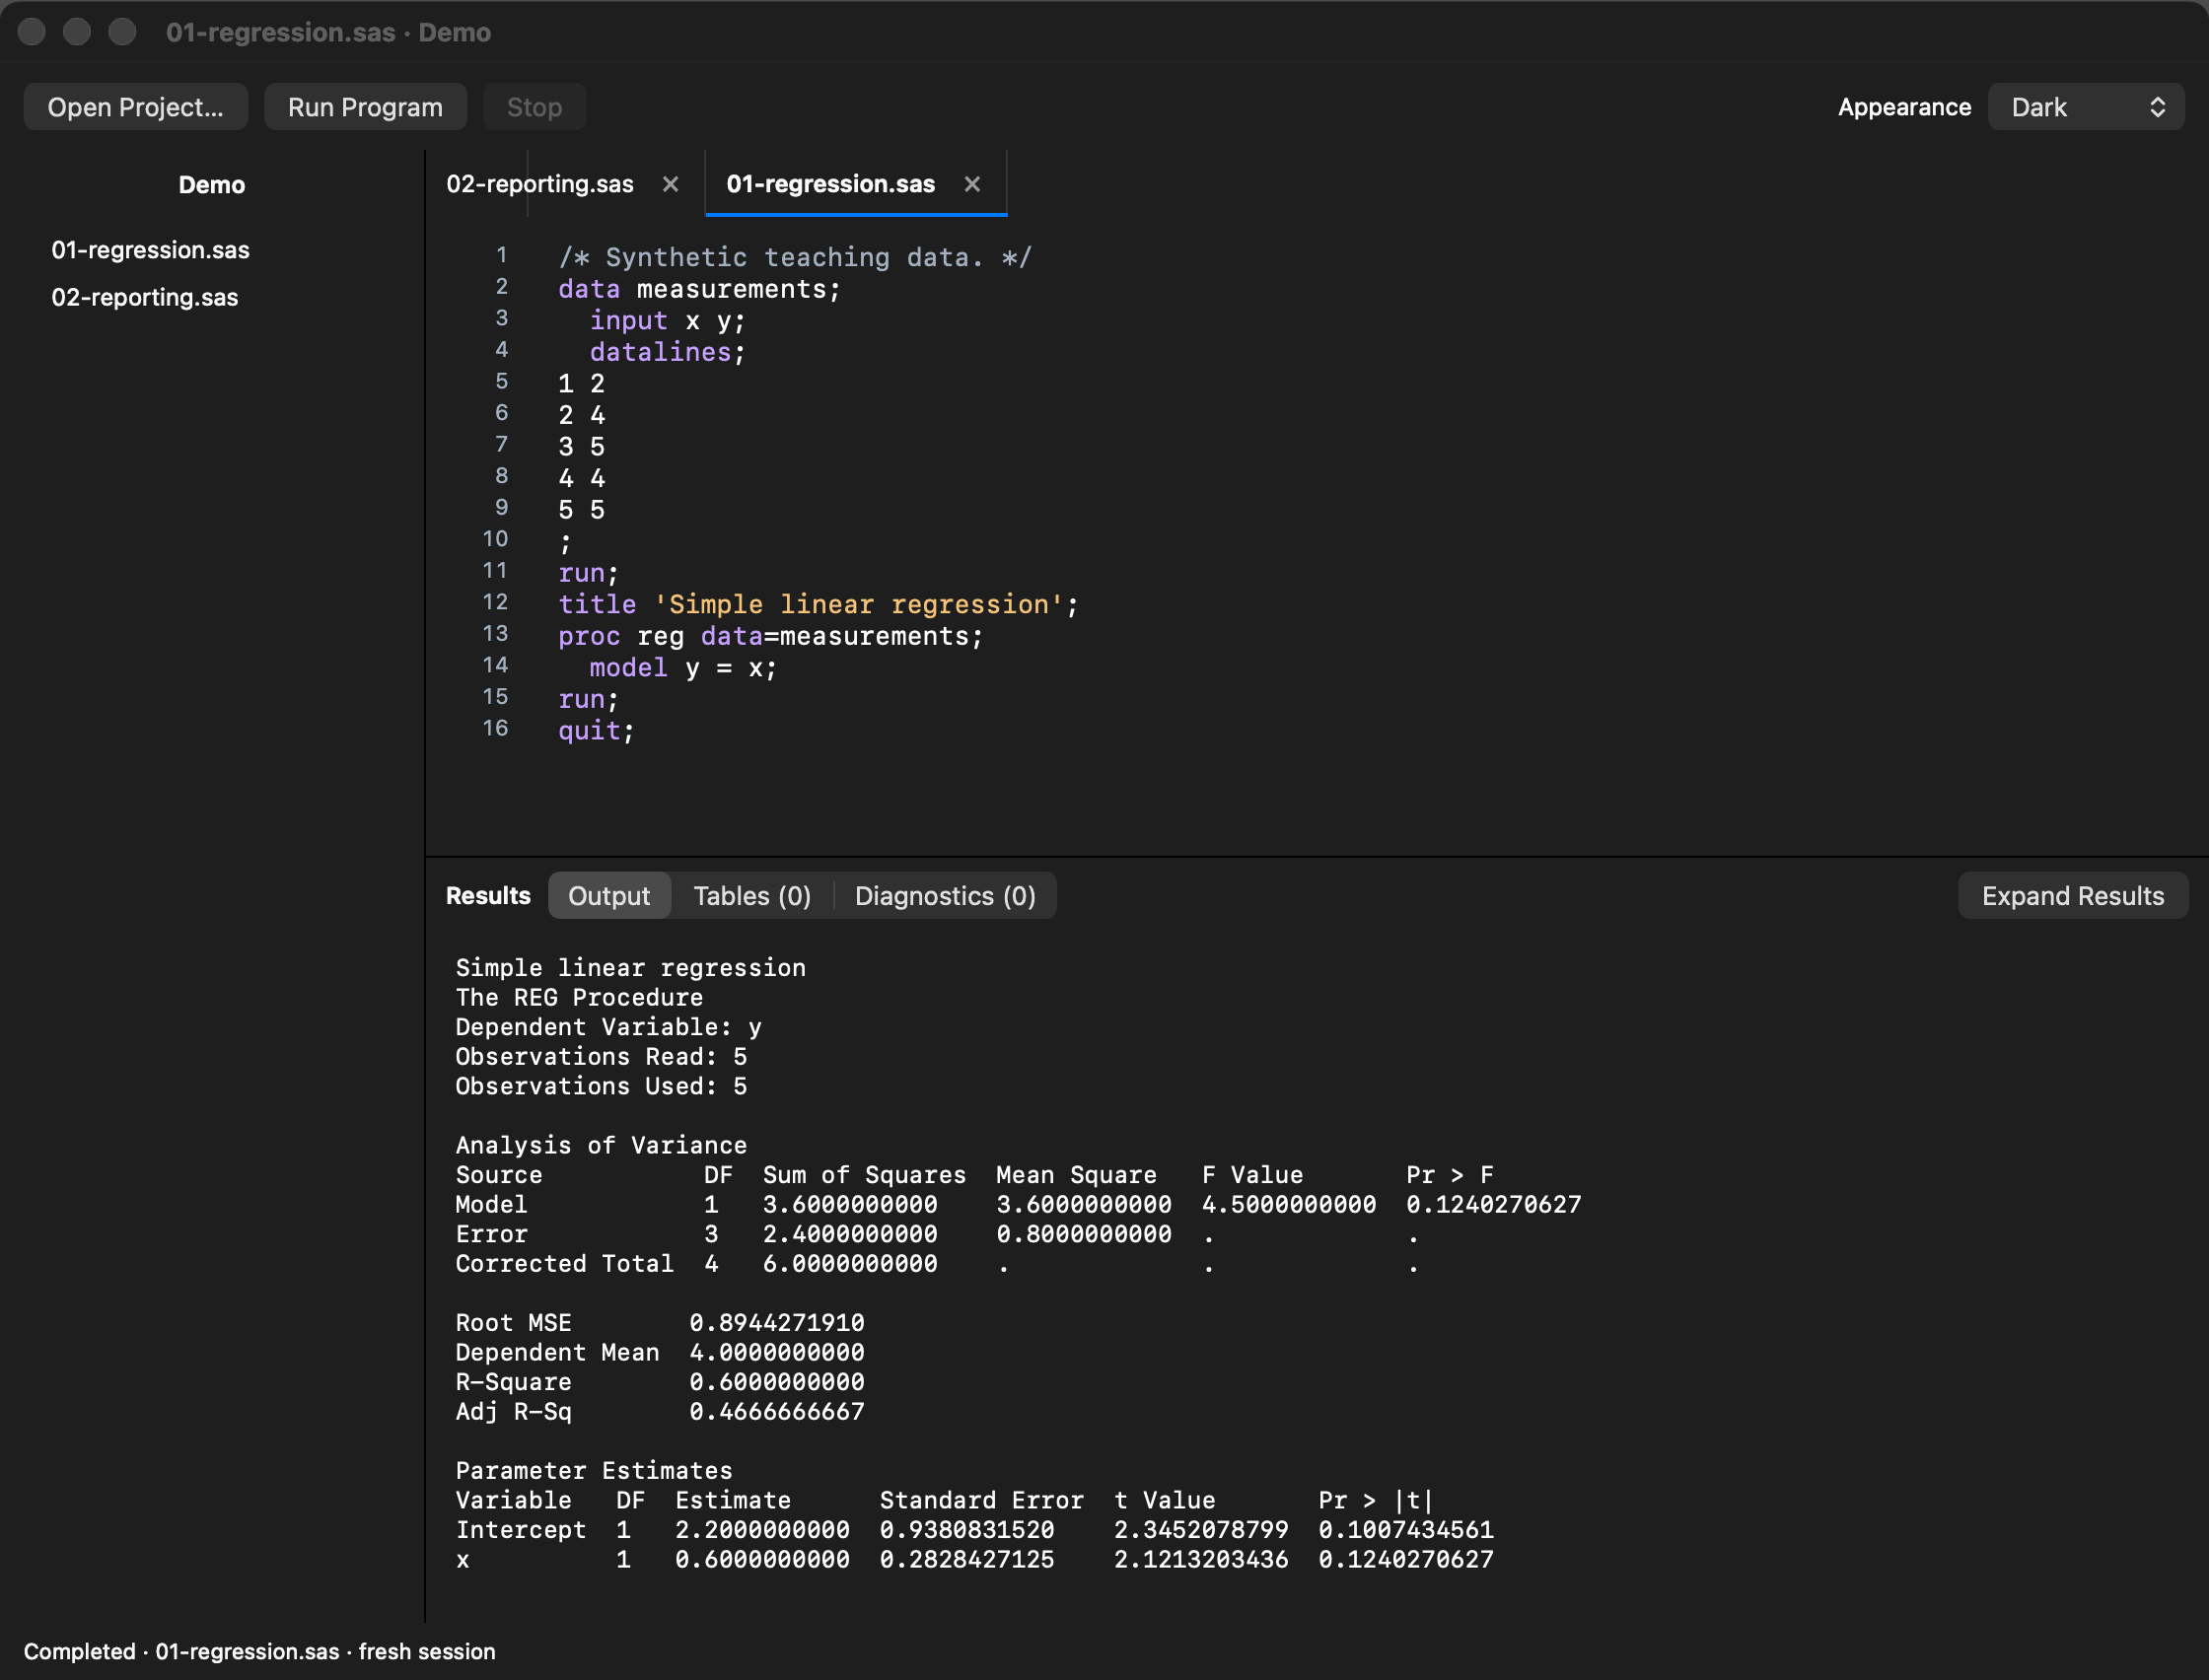
\includegraphics[width=\linewidth,height=5.65cm,keepaspectratio]{localstat-ide.png}
\end{column}
\end{columns}
\source{Source-rendered AppKit preview from commit 83b46a8; synthetic teaching data. Repository asset: localstat-ide.png.}
\note{Orient the professor to the sidebar, the two source tabs, the run controls, and the results tabs. The preview shows the current interface direction and a completed regression example. Explicitly identify it as a source-rendered preview rather than a live-session capture. The next slide enlarges the program and numerical result for readability. Suggested duration: 40 seconds.}
\end{frame}

% 5
\begin{frame}[fragile]{Regression example}
\relax
\begin{columns}[T,onlytextwidth]
\begin{column}{0.44\textwidth}
\begin{lstlisting}[style=sas]
data measurements;
  input x y;
  datalines;
1 2
2 4
3 5
4 4
5 5
;
run;
proc reg data=measurements;
  model y = x;
run;
quit;
\end{lstlisting}
\end{column}
\begin{column}{0.51\textwidth}
\point{Fitted model}{\[\widehat{y}=2.2+0.6x\]}
\vspace{-2mm}
\[R^2=0.600,\qquad n=5\]
\gap
{\small The implementation uses scaled, pivoted Householder QR.\par}
\gap
{\small Current scope: numeric predictors, an intercept, and complete-case OLS.}
\end{column}
\end{columns}
\source{Sources: synthetic example in localstat-ide.png; docs/COMPATIBILITY.md; docs/paper/localstat.tex.}
\note{Explain that this is deliberately small synthetic data, suitable for checking the fitted line by hand. The mean of x is 3 and the mean of y is 4. The cross-product sum is 6 and centered x sum of squares is 10, giving slope 0.6 and intercept 2.2. The model explains 3.6 of the total 6.0 sum of squares, so R-square is 0.6. Avoid interpreting five synthetic observations as a scientific finding. Mention that singular designs and unsupported REG options fail explicitly. Suggested duration: 60 seconds.}
\end{frame}

% 6
\begin{frame}{Formatted tables}
\relax
\begin{columns}[c,onlytextwidth]
\begin{column}{0.30\textwidth}
\point{Table output}{PRINT, FREQ, and TABULATE results.}
\gap
\point{Native workflow}{View tables, print them, or include them in a PDF.}
\gap
{\small Light appearance shown.}
\end{column}
\begin{column}{0.67\textwidth}
\centering
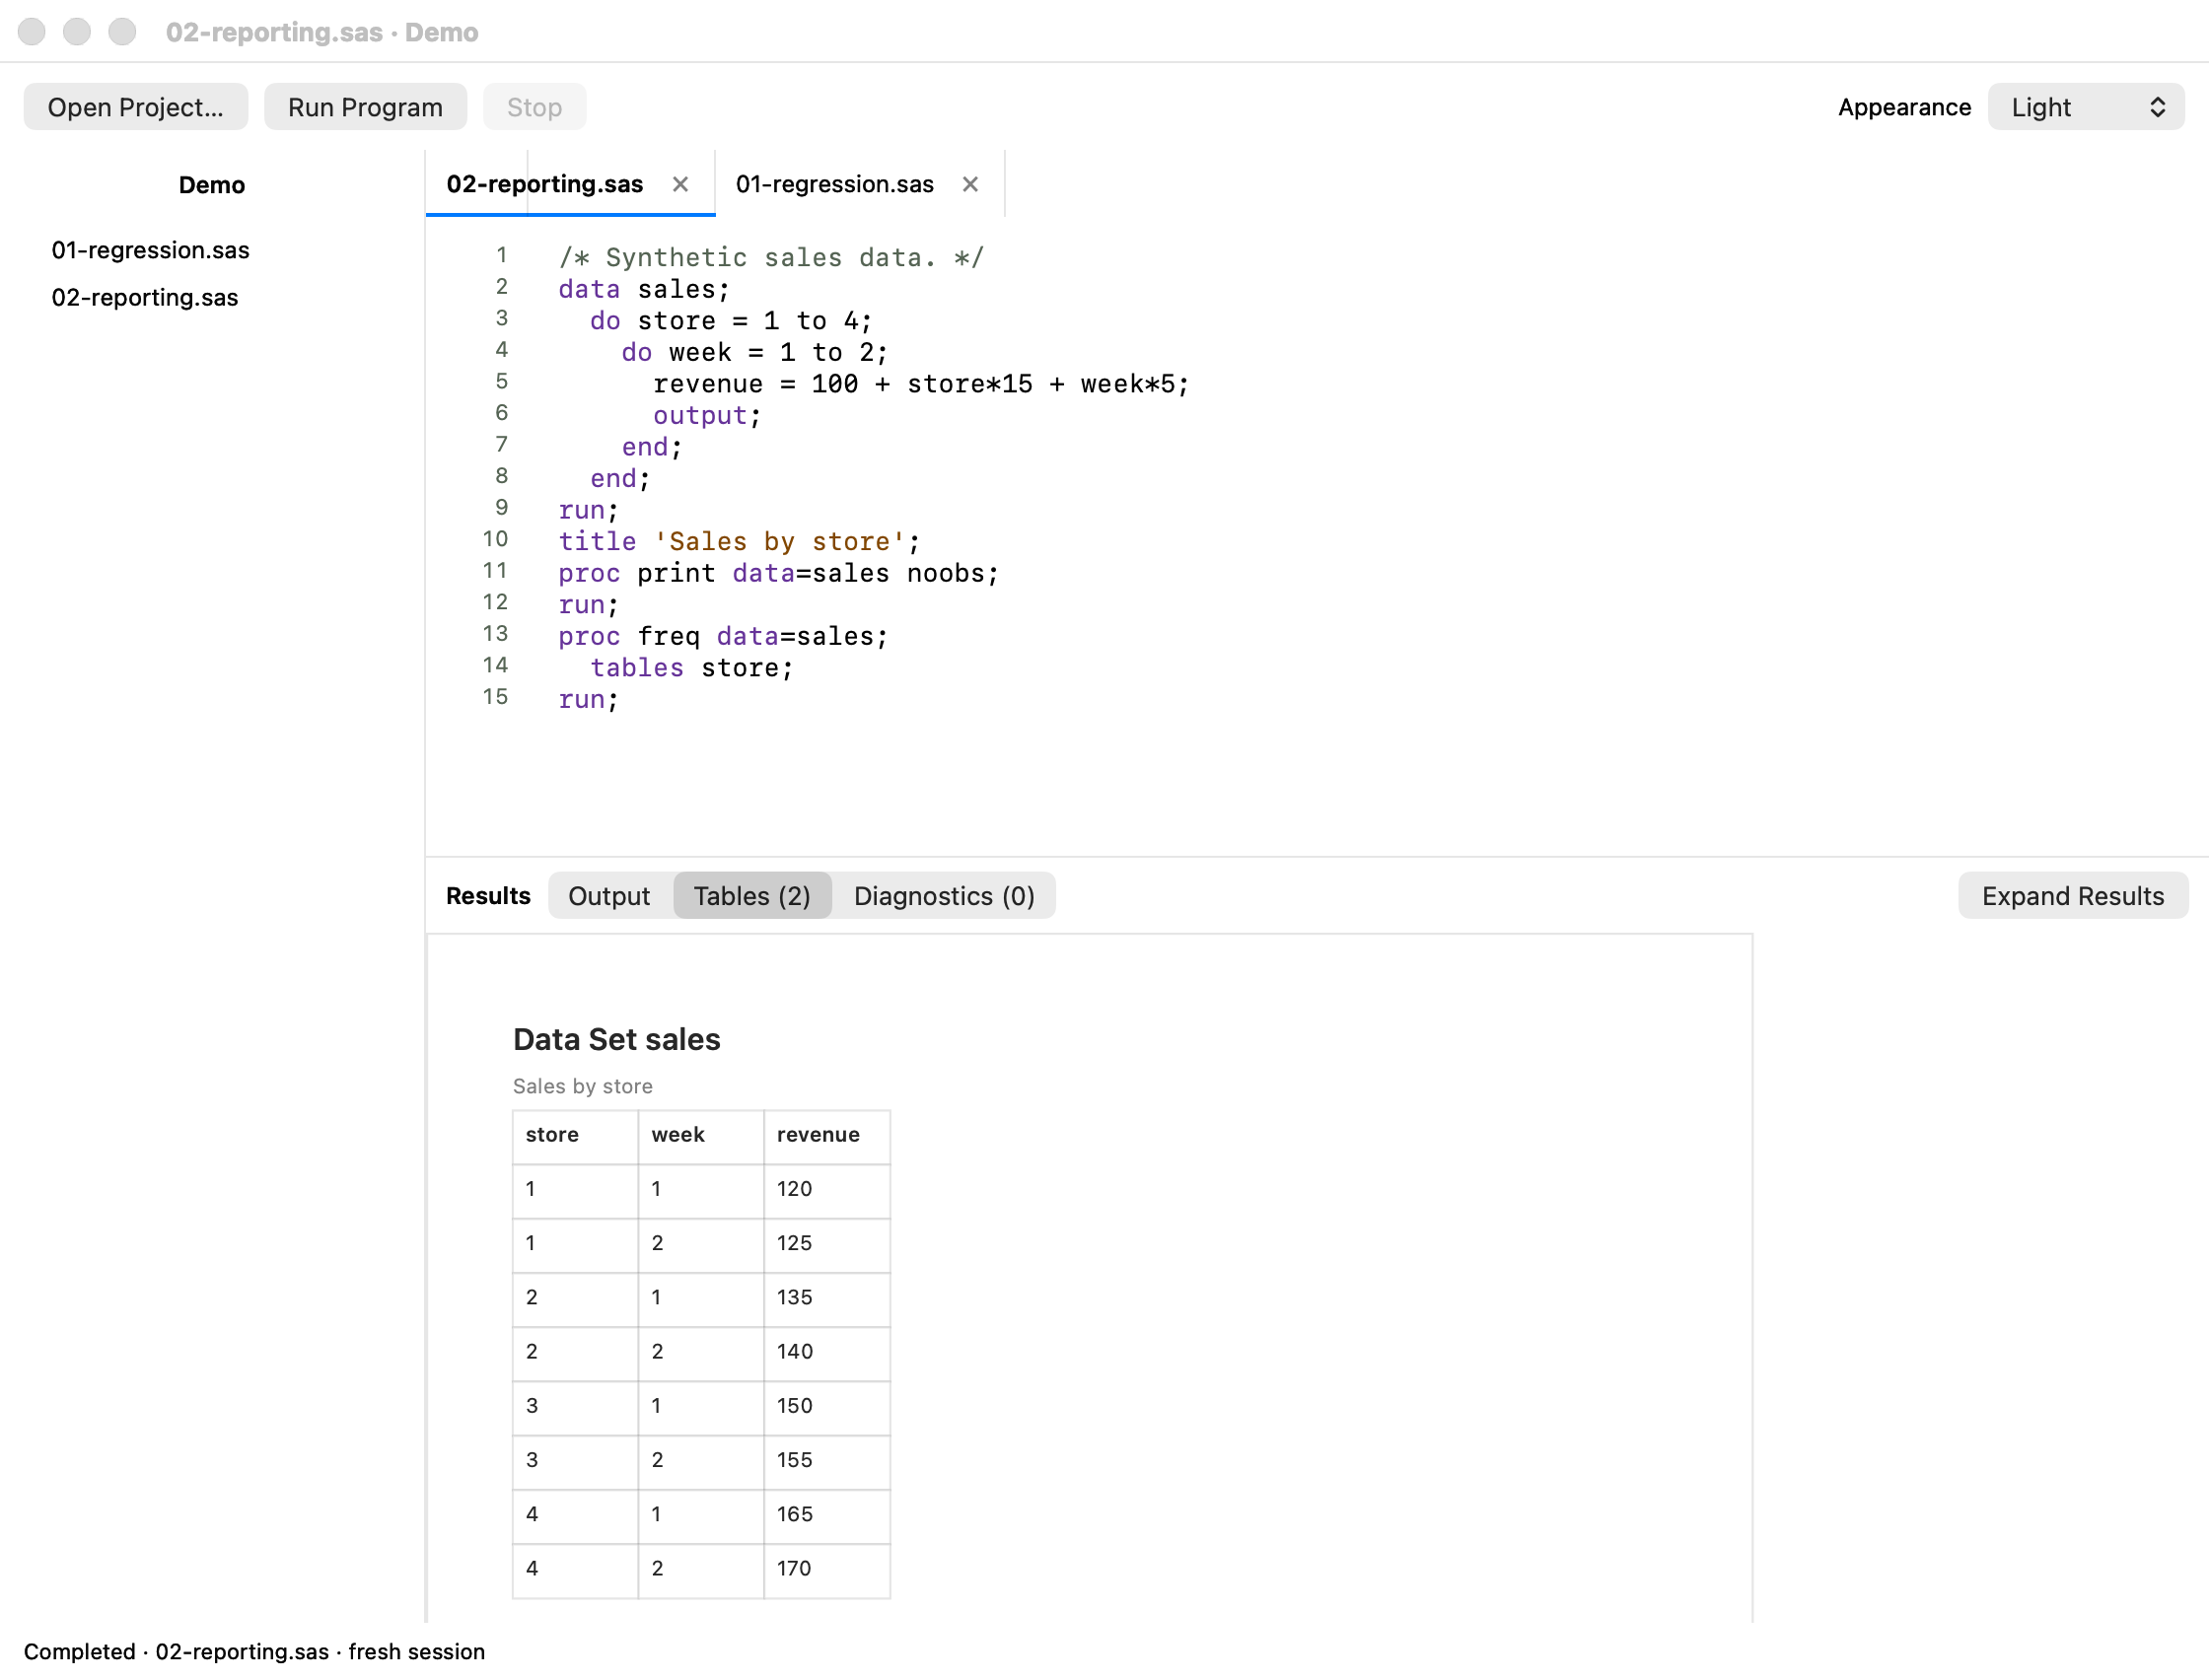
\includegraphics[width=\linewidth,height=5.65cm,keepaspectratio]{localstat-tables.png}
\end{column}
\end{columns}
\source{Source-rendered AppKit preview from commit 83b46a8; eight synthetic sales rows. Repository asset: localstat-tables.png.}
\note{The source program creates four stores with two weeks per store. PRINT creates the displayed table and FREQ creates another result, reflected in two formatted output tables. This illustrates the structured-table path rather than parsing aligned text into a guessed schema. The 0.1.3-alpha build includes this view. Suggested duration: 40 seconds.}
\end{frame}

% 7
\begin{frame}{Searchable PDF reports}
\relax
\centering
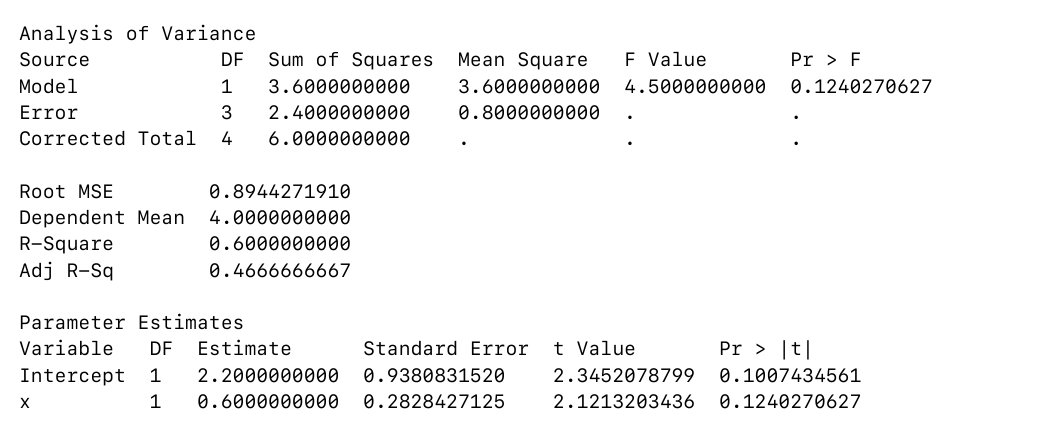
\includegraphics[width=0.98\linewidth,height=4.7cm,keepaspectratio]{localstat-pdf-output.png}\par
\vspace{2mm}
\raggedright
{\small Report includes source, metadata, results and diagnostics.\par}
\source{Rendered PDF excerpt: localstat-pdf-output.png. IDE report export; SAS ODS PDF remains unsupported. Sources: README; docs/COMPATIBILITY.md.}
\note{Point out aligned ANOVA columns, model statistics, and the parameter estimates. The PDF preserves the source that actually ran, including an unsaved editor snapshot. It is searchable and paginated. This is an application report export, not an implementation of the SAS ODS PDF destination. Suggested duration: 40 seconds.}
\end{frame}

% 8
\begin{frame}{Verification evidence}
\relax
\small
\renewcommand{\arraystretch}{1.15}
\begin{tabular}{@{}p{0.34\textwidth}p{0.59\textwidth}@{}}
\toprule
\textbf{Recorded suite} & \textbf{Coverage} \\
\midrule
973 runtime unit tests & Interpreter behavior and regressions \\
1,924 corpus programs & Language and procedure fixtures \\
11 end-to-end programs & Complete program execution \\
75 Swift tests & App, editor and reports; one opt-in skip \\
\bottomrule
\end{tabular}\par
\vspace{4mm}
{\small Analytical numerical checks and published examples support correctness for tested cases. Direct installed-SAS comparison remains future work.}
\source{Source: docs/VERIFICATION.md, current integration record dated 5 November 2026. Counts reflect the recorded suite, not a new run for this deck.}
\note{Distinguish software regression evidence from full language conformance. The maintained verification record is newer than the summary counts in the README, so these counts follow the dated verification document. A successful fixture does not establish universal SAS equivalence. Numerical checks include analytical coefficients and a published SAS example with stated tolerances. No installed SAS engine was used for direct comparison. Suggested duration: 50 seconds.}
\end{frame}

% 9
\begin{frame}{Interpreter memory results}
\relax
{\small Controlled before/after study, 4 November 2026.\par
Apple M5, 16 GB RAM; 15 measured repetitions per build and configuration.\par}
\vspace{3mm}
\small
\renewcommand{\arraystretch}{1.15}
\begin{tabular}{@{}lrrr@{}}
\toprule
\textbf{1 million rows} & \textbf{Before} & \textbf{After} & \textbf{Reduction} \\
\midrule
CSV round trip & 2324.0 & 579.7 & 75.1\% \\
FREQ & 1464.5 & 357.8 & 75.6\% \\
SQL join & 2005.5 & 921.7 & 54.0\% \\
\bottomrule
\end{tabular}\par
\vspace{4mm}
{\small Median peak interpreter RSS in MiB. Across seven numeric workload families, reductions range from 54.0\% to 75.6\%.}
\source{Source: docs/paper/results/2026-11-04-optimization/memory-comparison.tex and experiment README. Native app peak memory was not measured.}
\note{The comparison interleaved the CLI builds and counterbalanced native runs. It records 1,406 CLI observations and 506 native observations, including first executions and warmups. These rows are selected from the seven million-row numeric workload families, not all available workloads or real-world SAS programs. The runtime changes reclaim CSV scratch storage and avoid redundant retained row allocations. Ratios compare medians. The study does not isolate the effect of each individual change. Suggested duration: 70 seconds.}
\end{frame}

% 10
\begin{frame}{PRINT latency results}
\relax
\small
\renewcommand{\arraystretch}{1.15}
\begin{tabular}{@{}p{0.42\textwidth}rrr@{}}
\toprule
\textbf{Measured path} & \textbf{Before} & \textbf{After} & \textbf{Ratio} \\
\midrule
PRINT 10,000: table build & 210.5 & 51.8 & $4.07\times$ \\
PRINT 10,000: whole app & 343.5 & 172.9 & $1.99\times$ \\
DATA 10,000: whole app & 74.2 & 74.9 & $0.99\times$ \\
\bottomrule
\end{tabular}\par
\vspace{4mm}
{\small Median milliseconds; 15 measured observations per cell. Cached text measurements reduce table construction work.\par}
\gap
{\small All 10,000 PRINT rows remain on 385 pages. The DATA app case shows little change.}
\source{Source: native-comparison.tex and experiment README in docs/paper/results/2026-11-04-optimization/. Ratio = before median / after median.}
\note{Separate table construction from whole-app latency. The former starts with a preloaded validated table and excludes interpreter execution, JSON decoding, and drawing. The app path includes result application, layout, a synchronous display pass, and one-millisecond observation polling. It does not measure physical screen presentation. PRINT app IQR widths are 41.4 ms before and 5.8 ms after. Table-build IQR widths are 11.3 and 1.8 ms. DATA app IQR widths are 1.1 and 1.5 ms. No significance test, confidence interval, or causal per-change ablation is claimed. Suggested duration: 70 seconds.}
\end{frame}

% 11
\begin{frame}{Current limitations}
\relax
\begin{itemize}
\setlength{\itemsep}{3mm}
\item Partial language coverage. GLM, LOGISTIC, MIXED and other modeling procedures remain unsupported.
\item WORK and macro state reset on every run. Output arrives after execution finishes.
\item Programs use the app's filesystem permissions. The alpha is unsandboxed, ad-hoc signed and unnotarized.
\item Evaluation uses one Mac and synthetic workloads. Direct SAS-engine comparison remains incomplete.
\end{itemize}
\source{Sources: docs/COMPATIBILITY.md; docs/VERIFICATION.md; optimization experiment README. Screenshots predate the 0.1.3-alpha interface style.}
\note{Keep the boundaries explicit. The current regression subset rejects singular designs rather than reproducing SAS generalized-inverse handling. There is no persistent interactive session or SAS graphics. Screenshots show an earlier interface style, while the 0.1.3-alpha build includes the demonstrated functions. The local process boundary resets state but does not sandbox untrusted code. Suggested duration: 60 seconds.}
\end{frame}

% 12
\begin{frame}{Discussion with the professor}
\relax
\point{Proposed next evaluation}{Compare course programs against an installed SAS engine using explicit numerical tolerances.}
\gap
\point{Usability study}{Observe students editing a program and exporting its results.}
\gap
\point{Feedback requested}{Which exercises and compatibility gaps should guide the next iteration?}
\source{Proposed future work for discussion. Repository and evidence: \href{https://github.com/hafiz122/localstat}{github.com/hafiz122/localstat}.}
\note{Present these as proposals, not completed studies or agreed commitments. Ask the professor to help identify a small set of representative course exercises and an appropriate reference SAS installation. Useful feedback includes whether the project should emphasize systems engineering, numerical validation, or student workflow. This is the end of the main presentation. Suggested duration: 45 seconds plus discussion.}
\end{frame}

\appendix

% 13
\begin{frame}{Appendix: live demonstration}
\relax
\begin{enumerate}
\setlength{\itemsep}{3mm}
\item Open \texttt{01-regression.sas} and run the full program.
\item Check $\widehat{y}=2.2+0.6x$ and $R^2=0.600$ in Output.
\item Run \texttt{02-reporting.sas} and inspect Output Data.
\item Export a PDF, then open Compatibility and Limitations.
\end{enumerate}
\vspace{4mm}
{\small Included demo programs reproduce the synthetic examples shown in the screenshots.}
\source{Use 0.1.3-alpha or a current source build for formatted output data.}
\note{Allow about two minutes if the professor wants a demonstration. Use the demo directory included with the Beamer source package as the project folder. Set editor and output font sizes before screen sharing. Keep the slides available as a fallback. The expected FREQ table has four stores, each with frequency 2 and percent 25. The PRINT table contains eight rows.}
\end{frame}

% 14
\begin{frame}{Appendix: sources and reproducibility}
\relax
{\small
\point{Implementation and scope}{\texttt{README.md}, \texttt{docs/COMPATIBILITY.md},\\
\texttt{docs/VERIFICATION.md}, \texttt{docs/paper/localstat.tex}}
\vspace{1mm}
\point{Controlled study}{\texttt{docs/paper/results/2026-11-04-optimization/}\\
Raw observations, source archives and result tables.}
\vspace{1mm}
\point{Reproduction instructions}{\texttt{docs/paper/BENCHMARKS.md} and \texttt{docs/paper/README.md}}
\vspace{1mm}
\point{Image provenance}{App previews: source-rendered views, commit \texttt{83b46a8}.\\
PDF: rendered export excerpt. Example datasets are synthetic.}
}
\source{OpenSAS ancestry and preview provenance: project README and docs/RUNTIME\_CHANGES.md.}
\note{The paper preserves separate baseline and controlled optimization experiments. The evaluated working tree was not a clean released build; frozen source archives, source hashes, and executable hashes identify the evaluated artifacts. The public release and the current source should be treated separately. The recorded study supports its stated workload checks and does not establish general SAS equivalence or superiority over another language.}
\end{frame}

\end{document}
